\section{Semi-synthetic benchmarks and the \texttt{confounderalarm} package}
\label{sec:benchmarks}

The theory and simulation layers of the preceding sections rest on synthetic geometry. This section tests the calibrated alarm and the trim-then-regress recipe on real covariate geometry where ground truth is created by injection: a semi-synthetic design in the template of \citet{ulmer2025sdforest}, with real $X$, known $\beta/\gamma/f$ mechanism, and known $\tau$. Three families provide six frozen configurations (main and wide/sub cuts each). Family A is AddNeuroMed blood gene expression (GSE63060 and GSE63061 pooled \citep{geo_gse63060,geo_gse63061}, $717$ samples, $2000$ or $1800$ probes), whose dominant spectral structure is processing batch. Family B is the IHDP covariate benchmark \citep{hill2011bayesian} ($747$ rows) mapped through a seeded random-Fourier-feature expansion to $750$ or $150$ columns, receiving an injected dense confounder on real causal-benchmark geometry. Family C is the wooldridge k401ksubs household cross-section \citep{wooldridge2016introductory} ($800$-row seeded subsample, RFF-featurized to $1600$ or $160$ columns), which also carries the M2 treatment block with e401k as treatment and nettfa as outcome. Aspects span $c \in [0.20, 4.64]$ (the upper end is the single-batch A-sub cut, $n=388$, $p=1800$), and designs are fixed across injections so eigendecompositions are computed once per configuration.

A premise quantified before anything is injected: every unmodified design is massively outlier-positive against the white-noise Tracy--Widom threshold. The largest-eigenvalue TW statistics are $48{,}430.8$ for A-main, $8{,}360.0$ for C-main, $1{,}444.8$ for B-main, $1{,}191.0$ for C-wide, $308.8$ for B-wide, and $155.4$ even for the single-batch A-sub design. Scree inspection therefore rejects ``white noise'' on all six designs before any confounding exists. Four findings were predeclared and registered before any benchmark data were generated, and we label them PF-1 (frontier straddle), PF-2 (scree false alarms), PF-3 (trim-then-regress), and PF-4 (calibration versus informality); subsections below report PF-2 first because its premise, that spectrum-gazing itself carries no confounding signal on these designs, motivates every other measurement.

\subsection*{PF-2: spectrum-gazing is not evidence}

On every unmodified design, every matched-null twin (which shares seeds and drops only the $f\gamma$ link from $Y$), and every permutation null, the S0 scree test at the 99th Tracy--Widom percentile rejects with rate exactly $1.000$. The scree statistic responds to design structure, not to confounding: it cannot distinguish a batch-dominant expression matrix from a confounded one. This quantifies, with matched-null rates, the claim that ``I checked the spectrum'' carries zero evidential weight about hidden dense confounding, and it is why the alarm below calibrates against matched twins of the realized design rather than against white noise.

\subsection*{PF-1: power straddles each family's own predicted frontier}

The frozen alarm (statistic S2-bench, the packaged variant of S2 that re-estimates its nuisance scales on each benchmark configuration; amended before any calibration data after smoke testing exposed response-scale suppression and a bulk-shape mismatch on family A) standardizes per-coordinate spectral correlations between $X'Y$ directions and top sample eigenvectors using twin-estimated null scales, thresholds the maximum by a matched-null Monte Carlo quantile, and ships a predicted frontier $g^*$ from the capture-weighted slope law of Section~\ref{sec:detection}. Table~\ref{tab:pf1} reports the straddle test on all six configurations: power at half the predicted frontier lies in $[0.14, 0.21]$ (requirement $\le 0.25$) and power at twice the frontier between $0.975$ and $1.00$ (requirement $\ge 0.80$). In-sample matched-null size equals $0.05$ by construction, and the out-of-sample split-half twin-geometry control holds at $0.000$ to $0.003$. Empirical 80\%-power points sit between one and two times the prediction on every family, with ratios near $1.4$, consistent with the Phase-2 experience that the frontier law is accurate to well within a factor of $1.5$.

\begin{table}[t]
\centering
\caption{PF-1 straddle across the six benchmark configurations. $g^*$ is the predicted frontier; powers are rejection frequencies at multiples of $g^*$; the split-half column is the out-of-sample twin-geometry negative control.}
\label{tab:pf1}
\begin{tabular}{lccccc}
\toprule
Config & $g^*$ & Power $(0.5\times)$ & Power $(1\times)$ & Power $(2\times)$ & Split-half size \\
\midrule
A\_main & 0.762 & 0.143 & 0.480 & 0.998 & 0.000 \\
A\_sub  & 0.511 & 0.158 & 0.543 & 0.990 & 0.000 \\
B\_main & 1.012 & 0.163 & 0.553 & 0.983 & 0.000 \\
B\_wide & 1.062 & 0.155 & 0.523 & 0.975 & 0.000 \\
C\_main & 1.663 & 0.190 & 0.515 & 0.978 & 0.000 \\
C\_wide & 1.764 & 0.205 & 0.548 & 0.995 & 0.003 \\
\bottomrule
\end{tabular}
\end{table}

We record the gate mechanics transparently. The literal mechanical check, requiring control rejections inside the predeclared $[0.02, 0.10]$ band, failed on all six configurations because every control size sits below the lower edge ($0.000$ to $0.003$): the controls are conservative, never anti-conservative, across more than $3{,}000$ control evaluations. The mechanism is understood rather than waved away; permutation removes the beta-leakage component of the twin-null coordinate variances, shrinking the standardized statistic, and split-half evaluation halves the leakage mass outright. Because the band's predeclared purpose was detecting miscalibration in the dangerous direction, and the dangerous direction never fires, the literal band check failed only from below and was recorded as requiring review; a written adjudication documents why a conservative direction does not indicate miscalibration, and the verdict is GO. After a concurrency fault in its first pass, the C-main null configuration was rerun in full; its frozen Monte Carlo quantile reproduced to a $0.00\%$ shift, and all thresholds were audited against this rerun.

\subsection*{PF-3: trim-then-regress on real econometric geometry}

In the C-main M2 block ($\tau_{\mathrm{true}} = 1$, sparse treatment projection, injected factor loading $\|\delta\| = 0.3$), OLS mean absolute $\tau$ error inflates to $0.421$ under a one-times-frontier injection, while Onatski-trimmed regression holds at $0.173$: a ratio of $2.43$, with the correct sign recovered in $100\%$ of replications. The cost of trimming under the clean null arm is negligible ($0.128$ versus $0.110$ for OLS). Ridge at unit penalty lands between ($0.238$). This validates on real geometry the recipe that survives the negative result of Section~\ref{sec:estimation}: hard Onatski trimming rather than tuned soft weights, on geometry that was not manufactured by our simulator.

\subsection*{PF-4: calibration versus informality, head to head}

On identical data and identical controls we compared the alarm against incumbent spectral diagnostics: the response-aware confounding-strength proxy of \citet{rendsburg2024consistent} (estimated under the uncorrelated-confounder model), with permutation bootstrap thresholding \citep{rendsburg2024consistent}, a Janzing--Sch{\"o}lkopf-style spectral asymmetry score with permutation calibration \citep{janzing2018detecting}, Tracy--Widom scree, and partial-$F$ tests on principal-component scores. Both proxy methods do track the injected strength monotonically across arms; their point estimates order correctly. What they lack is any valid threshold off the calibration distribution: evaluated out-of-sample on split-half controls, the strength proxy rejects under $H_0$ at rates $0.07$ to $0.92$ and the asymmetry score at $0.61$ to $1.00$, while the twin-calibrated alarm holds at $0.000$ to $0.003$. Partial-$F$ is uncalibrated on real geometry ($0.25$ to $0.93$), and scree alarms everywhere ($1.000$) because it fires on structure regardless of confounding. Table~\ref{tab:calib} summarizes what each method ships.

\begin{table}[t]
\centering
\caption{Calibration versus informality on identical benchmark data and controls. Out-of-sample control size is the realized rejection frequency under $H_0$ on split-half twin-geometry controls, pooled over the six configurations.}
\label{tab:calib}
\begin{tabular}{lccc}
\toprule
Method & Ships exact null law? & Predicted frontier? & Out-of-sample control size \\
\midrule
S2-bench alarm (ours) & Yes (matched-null MC) & Yes (capture-law $g^*$) & 0.000--0.003 \\
Strength proxy (Rendsburg et al.\ implementation of the Janzing--Sch{\"o}lkopf criterion), permutation bootstrap \citep{rendsburg2024consistent,janzing2018detecting} & No (approximate proxy) & No & 0.07--0.92 \\
JS-asym, perm.\ bootstrap & No (approximate transcription) & No & 0.61--1.00 \\
Scree TW99 & White-noise law only (wrong null) & No & 1.000 \\
Partial-$F$ on PC scores & Analytic $F$ (wrong null) & No & 0.25--0.93 \\
\bottomrule
\end{tabular}
\end{table}

\subsection*{Sensitivity findings, reported honestly}

Two sensitivity results qualify where the method works, and we report them as findings rather than burying them. First, concentrating the link on the dominant mega-spike direction reduces detectability: alignment power $0.05$ versus $0.48$ for the spread placement at the same $g^*$ on A-main, while concentrating on the second spike raises power to $0.865$. The mechanism is a leakage tax: the first coordinate's twin scale $s_1 = 36.6$ absorbs batch-direction noise that grows faster than the link's mean shift, so frontier prediction quality is alignment-dependent. Visibility depends on where the link rides, not only how strong it is, which strengthens the decoupling narrative but bounds the prediction layer's uniformity. Second, heteroskedastic response noise causes no material drift (powers $0.47$ to $0.58$ versus $0.48$ to $0.55$ baseline, calibration preserved), and adding one undetected injection direction dilutes power moderately (ranks-plus-one powers $0.28$ to $0.44$, no size inflation); dropping a direction on A-main reproduces the mega-spike mechanism (power $0.055$).

\subsection*{Reproducibility and the package}

The pipeline ships as \texttt{confounderalarm} v0.1.0, installable and exercised by three green unit tests, with a command-line interface (\texttt{python -m confounderalarm --csv ...}) and two worked examples in the README. Given $(Y, X)$ it runs the detection path and returns the alarm verdict with a calibrated p-value, estimates $(\hat r, \hat l_j, \hat c)$, the placement of the observed statistic relative to the predicted frontier $g^*$, and a blind-region certificate stating when non-rejection is uninformative. Given $(Y, D, X)$ it additionally returns a treatment-effect adjustment, and there it recommends Onatski hard-trim regression explicitly, not tuned soft weights, encoding the kill of Section~\ref{sec:estimation} as interface behavior. Trusted-result reproductions guard the plumbing: the k401k eligibility coefficient of $+9.41$ (the positive Poterba--Venti--Wise eligibility sign \citep{poterba1995do} under plain covariate adjustment), IHDP adjusted estimates at the experimental benchmark scale ($3.93$ adjusted versus approximately $4.0$ experimental), and AddNeuroMed batch-dominant structure (pooled TW statistic $48{,}431$ versus $155$ within batch 2). Every pass-2 arm was independently re-executed from the pinned repository tag on separate hardware: $41/41$ cells reproduce with maximum statistic deviation $7.7 \times 10^{-13}$ and zero rejection disagreements. Figure~\ref{fig:bench} displays the frontier check underlying PF-1.

\begin{figure}[t]
\centering
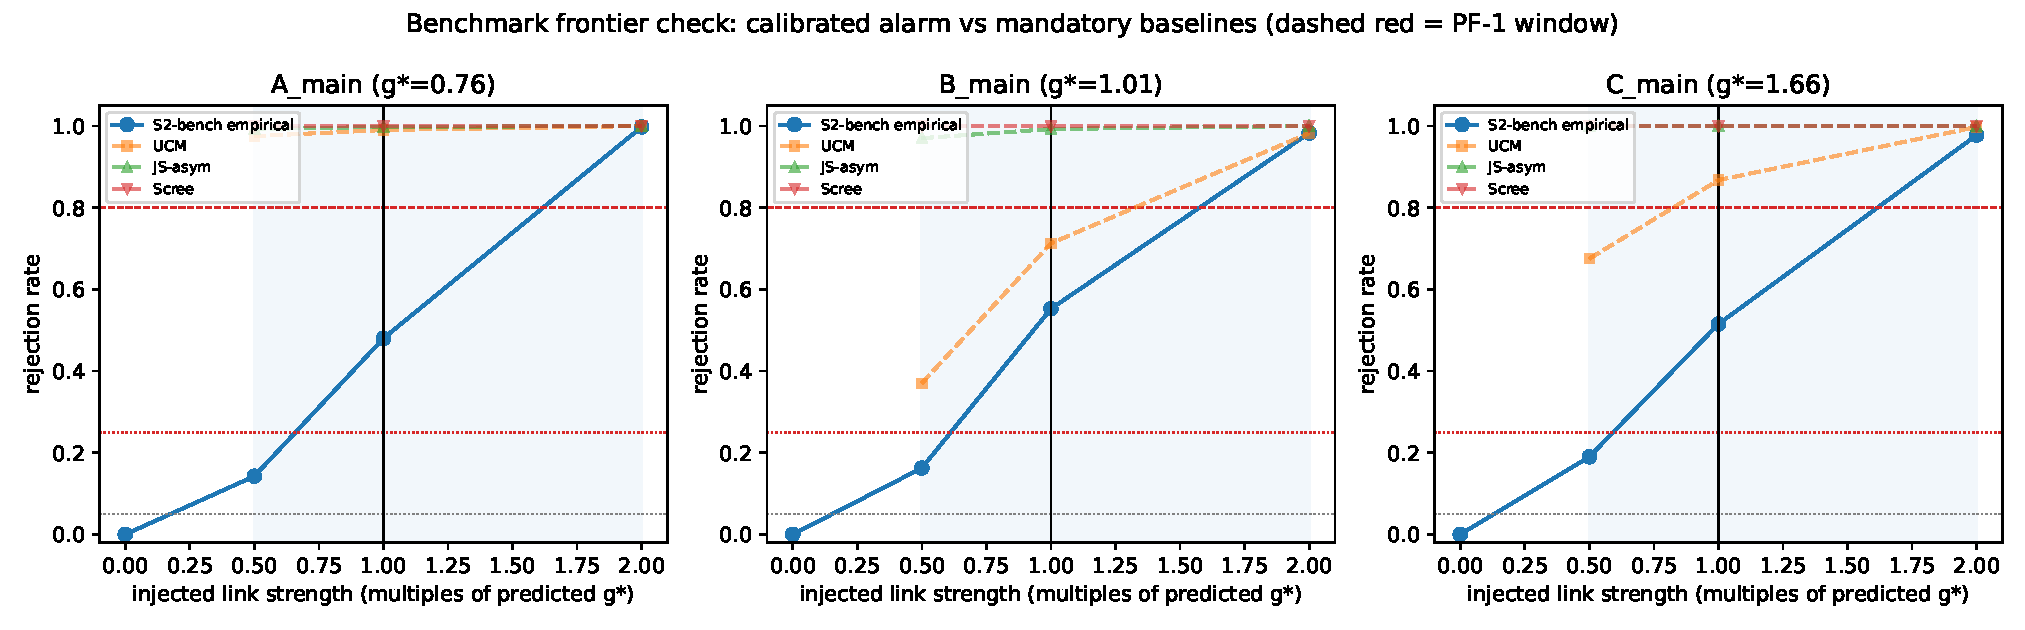
\includegraphics[width=\linewidth]{figures/benchmark_frontier_check.pdf}
\caption{Benchmark frontier check: empirical rejection curves against the predicted frontiers $g^*$ across the six configurations, with negative-control sizes marked at the origin. Power rises through the predicted frontier and saturates by twice $g^*$ on every family.}
\label{fig:bench}
\end{figure}


Every number in this section regenerates from frozen configurations with recorded hashes; the audit trail, commands, and checksum manifests are collected in Appendix~\ref{app:repro}.
